\documentclass[tikz,border=2mm]{standalone}
\usepackage[utf8]{inputenc}
\usepackage[T1]{fontenc}
\usepackage{tikz}
\usetikzlibrary{arrows.meta, positioning}
\usepackage{pgfplots}

\pgfplotsset{compat=1.18}

\begin{document}

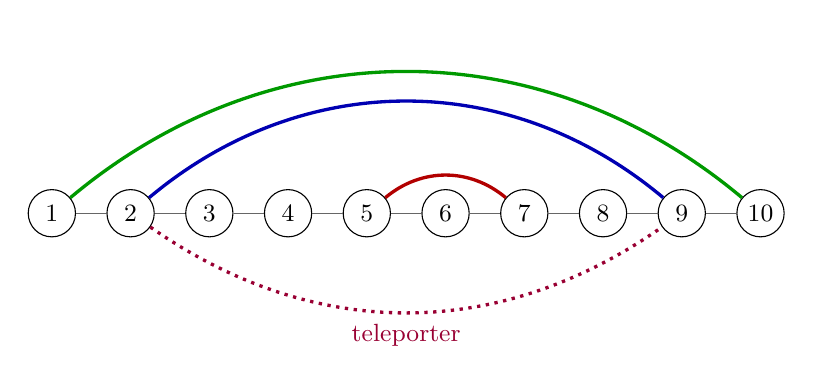
\begin{tikzpicture}[
    every node/.style={font=\small},
    hub/.style={circle, draw, minimum size=6mm, inner sep=0pt},
    route1/.style={very thick, green!60!black},
    route2/.style={very thick, blue!70!black},
    route3/.style={very thick, red!70!black},
    teleporter/.style={very thick, dotted, purple!80!black},
]

% Hubs on a line
\foreach \x in {1,...,10} {
    \node[hub] (n\x) at (\x,0) {\x};
}

% Tree edges
\foreach \x in {1,...,9} {
    \draw[black!60] (n\x) -- (n\the\numexpr\x+1\relax);
}

% Optimal teleporter placement
\draw[teleporter, bend right=35]
    (n2) to node[below, pos=0.5] {teleporter} (n9);

% (s,t) pairs
\draw[route1] (n1) to[bend left=40] (n10);
\draw[route2] (n2) to[bend left=40] (n9);
\draw[route3] (n5) to[bend left=40] (n7);

\end{tikzpicture}

\end{document}
